\documentclass{standalone}
\usepackage{tikz}
\usetikzlibrary{patterns, positioning}


\begin{document}
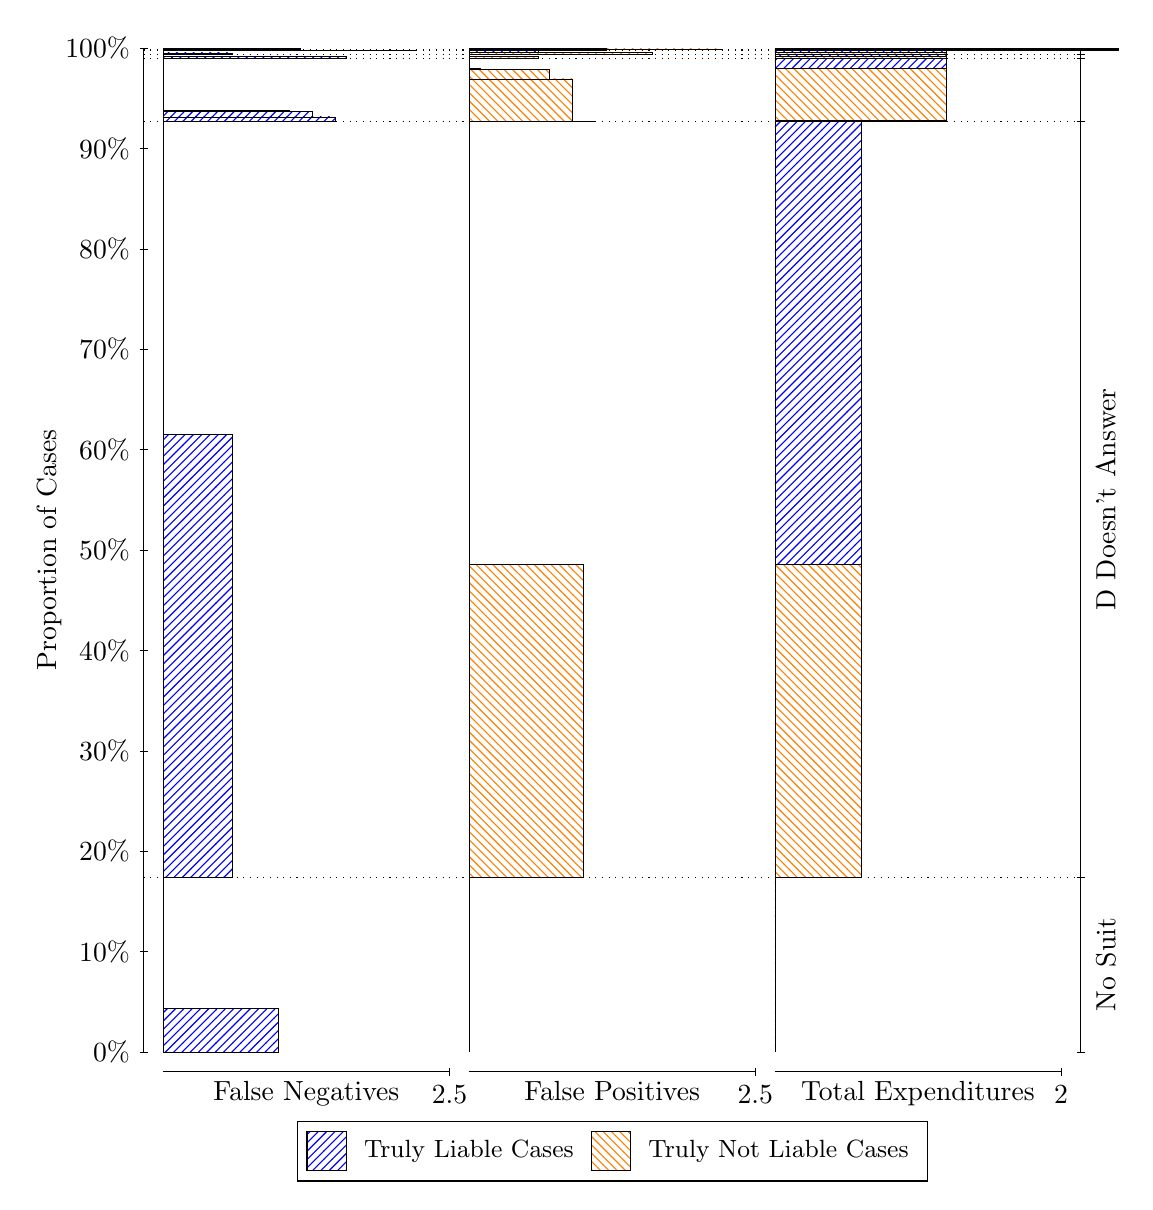
\begin{tikzpicture}
\draw[black, very thin] (1.5,1.75) -- (1.5,14.5);
\node[rotate=90, text=black, anchor=center] at (0.3, 8.125) {Proportion of Cases};
\draw[black, very thin] (1.45,1.75) -- (1.55,1.75);
\node[text=black, anchor=east] at (1.45, 1.75) {0\%};
\draw[black, very thin] (1.45,3.025) -- (1.55,3.025);
\node[text=black, anchor=east] at (1.45, 3.025) {10\%};
\draw[black, very thin] (1.45,4.3) -- (1.55,4.3);
\node[text=black, anchor=east] at (1.45, 4.3) {20\%};
\draw[black, very thin] (1.45,5.575) -- (1.55,5.575);
\node[text=black, anchor=east] at (1.45, 5.575) {30\%};
\draw[black, very thin] (1.45,6.85) -- (1.55,6.85);
\node[text=black, anchor=east] at (1.45, 6.85) {40\%};
\draw[black, very thin] (1.45,8.125) -- (1.55,8.125);
\node[text=black, anchor=east] at (1.45, 8.125) {50\%};
\draw[black, very thin] (1.45,9.4) -- (1.55,9.4);
\node[text=black, anchor=east] at (1.45, 9.4) {60\%};
\draw[black, very thin] (1.45,10.675) -- (1.55,10.675);
\node[text=black, anchor=east] at (1.45, 10.675) {70\%};
\draw[black, very thin] (1.45,11.95) -- (1.55,11.95);
\node[text=black, anchor=east] at (1.45, 11.95) {80\%};
\draw[black, very thin] (1.45,13.225) -- (1.55,13.225);
\node[text=black, anchor=east] at (1.45, 13.225) {90\%};
\draw[black, very thin] (1.45,14.5) -- (1.55,14.5);
\node[text=black, anchor=east] at (1.45, 14.5) {100\%};

\draw[black, very thin] (13.4,1.75) -- (13.4,14.5);
\draw[black, very thin] (13.35,1.75) -- (13.45,1.75);
\node[anchor=west] at (13.35, 1.75) {};
\draw[black, very thin] (13.35,3.9694) -- (13.45,3.9694);
\node[anchor=west] at (13.35, 3.9694) {};
\draw[black, very thin] (13.35,13.564) -- (13.45,13.564);
\node[anchor=west] at (13.35, 13.564) {};
\draw[black, very thin] (13.35,14.371) -- (13.45,14.371);
\node[anchor=west] at (13.35, 14.371) {};
\draw[black, very thin] (13.35,14.42) -- (13.45,14.42);
\node[anchor=west] at (13.35, 14.42) {};
\draw[black, very thin] (13.35,14.466) -- (13.45,14.466);
\node[anchor=west] at (13.35, 14.466) {};
\draw[black, very thin] (13.35,14.483) -- (13.45,14.483);
\node[anchor=west] at (13.35, 14.483) {};
\draw[black, very thin] (13.35,14.5) -- (13.45,14.5);
\node[anchor=west] at (13.35, 14.5) {};

\draw[black, very thin, pattern color=blue, pattern=north east lines] (1.75,1.75) rectangle (3.2033,2.3045);
\draw[black, very thin, pattern color=orange, pattern=north west lines] (1.75,2.3045) rectangle (1.75,3.9694);
\draw[black, very thin, pattern color=blue, pattern=north east lines] (1.75,3.9694) rectangle (2.622,9.5894);
\draw[black, very thin, pattern color=orange, pattern=north west lines] (1.75,9.5894) rectangle (1.75,13.564);
\draw[black, very thin, pattern color=blue, pattern=north east lines] (1.75,13.564) rectangle (3.93,13.625);
\draw[black, very thin, pattern color=blue, pattern=north east lines] (1.75,13.625) rectangle (3.6393,13.692);
\draw[black, very thin, pattern color=blue, pattern=north east lines] (1.75,13.692) rectangle (3.3487,13.705);
\draw[black, very thin, pattern color=orange, pattern=north west lines] (1.75,13.705) rectangle (1.75,14.371);
\draw[black, very thin, pattern color=blue, pattern=north east lines] (1.75,14.371) rectangle (4.0753,14.395);
\draw[black, very thin, pattern color=orange, pattern=north west lines] (1.75,14.395) rectangle (1.75,14.42);
\draw[black, very thin, pattern color=blue, pattern=north east lines] (1.75,14.42) rectangle (2.622,14.439);
\draw[black, very thin, pattern color=orange, pattern=north west lines] (1.75,14.439) rectangle (1.75,14.466);
\draw[black, very thin, pattern color=blue, pattern=north east lines] (1.75,14.466) rectangle (4.9473,14.472);
\draw[black, very thin, pattern color=orange, pattern=north west lines] (1.75,14.472) rectangle (1.75,14.483);
\draw[black, very thin, pattern color=blue, pattern=north east lines] (1.75,14.483) rectangle (3.494,14.495);
\draw[black, very thin, pattern color=orange, pattern=north west lines] (1.75,14.495) rectangle (1.75,14.5);
\draw[black, very thin, pattern color=orange, pattern=north west lines] (5.6333,1.75) rectangle (5.6333,3.415);
\draw[black, very thin, pattern color=blue, pattern=north east lines] (5.6333,3.415) rectangle (5.6333,3.9694);
\draw[black, very thin, pattern color=orange, pattern=north west lines] (5.6333,3.9694) rectangle (7.0867,7.9436);
\draw[black, very thin, pattern color=blue, pattern=north east lines] (5.6333,7.9436) rectangle (5.6333,13.564);
\draw[black, very thin, pattern color=orange, pattern=north west lines] (5.6333,13.564) rectangle (7.232,13.567);
\draw[black, very thin, pattern color=orange, pattern=north west lines] (5.6333,13.567) rectangle (6.9413,14.108);
\draw[black, very thin, pattern color=orange, pattern=north west lines] (5.6333,14.108) rectangle (6.6507,14.23);
\draw[black, very thin, pattern color=blue, pattern=north east lines] (5.6333,14.23) rectangle (5.7787,14.243);
\draw[black, very thin, pattern color=blue, pattern=north east lines] (5.6333,14.243) rectangle (5.6333,14.371);
\draw[black, very thin, pattern color=orange, pattern=north west lines] (5.6333,14.371) rectangle (6.5053,14.396);
\draw[black, very thin, pattern color=blue, pattern=north east lines] (5.6333,14.396) rectangle (5.6333,14.42);
\draw[black, very thin, pattern color=orange, pattern=north west lines] (5.6333,14.42) rectangle (7.9587,14.448);
\draw[black, very thin, pattern color=blue, pattern=north east lines] (5.6333,14.448) rectangle (6.5053,14.466);
\draw[black, very thin, pattern color=orange, pattern=north west lines] (5.6333,14.466) rectangle (7.3773,14.477);
\draw[black, very thin, pattern color=blue, pattern=north east lines] (5.6333,14.477) rectangle (5.924,14.483);
\draw[black, very thin, pattern color=orange, pattern=north west lines] (5.6333,14.483) rectangle (8.8307,14.488);
\draw[black, very thin, pattern color=blue, pattern=north east lines] (5.6333,14.488) rectangle (7.3773,14.5);
\draw[black, very thin, pattern color=orange, pattern=north west lines] (9.5167,1.75) rectangle (9.5167,3.415);
\draw[black, very thin, pattern color=blue, pattern=north east lines] (9.5167,3.415) rectangle (9.5167,3.9694);
\draw[black, very thin, pattern color=orange, pattern=north west lines] (9.5167,3.9694) rectangle (10.607,7.9436);
\draw[black, very thin, pattern color=blue, pattern=north east lines] (9.5167,7.9436) rectangle (10.607,13.564);
\draw[black, very thin, pattern color=orange, pattern=north west lines] (9.5167,13.564) rectangle (11.697,13.567);
\draw[black, very thin, pattern color=blue, pattern=north east lines] (9.5167,13.567) rectangle (11.697,13.58);
\draw[black, very thin, pattern color=orange, pattern=north west lines] (9.5167,13.58) rectangle (11.697,14.243);
\draw[black, very thin, pattern color=blue, pattern=north east lines] (9.5167,14.243) rectangle (11.697,14.371);
\draw[black, very thin, pattern color=orange, pattern=north west lines] (9.5167,14.371) rectangle (11.697,14.396);
\draw[black, very thin, pattern color=blue, pattern=north east lines] (9.5167,14.396) rectangle (11.697,14.42);
\draw[black, very thin, pattern color=orange, pattern=north west lines] (9.5167,14.42) rectangle (11.697,14.448);
\draw[black, very thin, pattern color=blue, pattern=north east lines] (9.5167,14.448) rectangle (11.697,14.466);
\draw[black, very thin, pattern color=orange, pattern=north west lines] (9.5167,14.466) rectangle (13.877,14.477);
\draw[black, very thin, pattern color=blue, pattern=north east lines] (9.5167,14.477) rectangle (13.877,14.483);
\draw[black, very thin, pattern color=orange, pattern=north west lines] (9.5167,14.483) rectangle (13.877,14.488);
\draw[black, very thin, pattern color=blue, pattern=north east lines] (9.5167,14.488) rectangle (13.877,14.5);
\draw[black, dotted] (1.5,3.9694) -- (13.4,3.9694);
\draw[black, dotted] (1.5,13.564) -- (13.4,13.564);
\draw[black, dotted] (1.5,14.371) -- (13.4,14.371);
\draw[black, dotted] (1.5,14.42) -- (13.4,14.42);
\draw[black, dotted] (1.5,14.466) -- (13.4,14.466);
\draw[black, dotted] (1.5,14.483) -- (13.4,14.483);
\draw[black, very thin] (1.75,1.5) -- (5.3833,1.5);
\node[text=black, anchor=north] at (3.5667, 1.5) {False Negatives};
\draw[black, very thin] (5.3833,1.45) -- (5.3833,1.55);
\node[text=black, anchor=north] at (5.3833, 1.45) {2.5};

\draw[black, very thin] (5.6333,1.5) -- (9.2667,1.5);
\node[text=black, anchor=north] at (7.45, 1.5) {False Positives};
\draw[black, very thin] (9.2667,1.45) -- (9.2667,1.55);
\node[text=black, anchor=north] at (9.2667, 1.45) {2.5};

\draw[black, very thin] (9.5167,1.5) -- (13.15,1.5);
\node[text=black, anchor=north] at (11.333, 1.5) {Total Expenditures};
\draw[black, very thin] (13.15,1.45) -- (13.15,1.55);
\node[text=black, anchor=north] at (13.15, 1.45) {2};

\node[text=black, centered, rotate=90] at (13.72, 2.8597) {No Suit};
\node[text=black, centered, rotate=90] at (13.72, 8.7665) {D Doesn't Answer};






\draw (7.449999999999999,1.5) node[draw=none] (baseCoordinate) {};
\begin{scope}[align=center]
        \matrix[scale=0.5, draw=black, below=0.5cm of baseCoordinate, nodes={draw}, column sep=0.1cm]{
            \node[rectangle, draw, minimum width=0.5cm, minimum height=0.5cm, pattern color=blue, pattern=north east lines] {}; &
            \node[draw=none, font=\small, text=black] (B) {Truly Liable Cases}; &
            \node[rectangle, draw, minimum width=0.5cm, minimum height=0.5cm, pattern color=orange, pattern=north west lines] {}; &
            \node[draw=none, font=\small, text=black] (B) {Truly Not Liable Cases}; \\
            };
\end{scope}

\end{tikzpicture}
\end{document}